\documentclass[12pt]{article}

\usepackage{sbc-template}

\usepackage{graphicx,url}
\usepackage{listings}


\usepackage[brazil]{babel}   
%\usepackage[latin1]{inputenc}  
\usepackage[utf8]{inputenc}  
% UTF-8 encoding is recommended by ShareLaTex

     
\sloppy

\title{Detector de concentração de álcool com base em
Arduíno}

\author{Luan S. Viana\inst{1},Maycon Rafael C. Borba\inst{2}, Lisandro Almeida\inst{3}}


\address{IFgoiano Campus Rio Verde-GO -- Bacharelado em Ciência da Computação}

\begin{document} 

\maketitle

\begin{abstract}
  This article will cover an embedded system
For detection of alcohol concentration based on Arduino, DSDetector, this system uses the paradigm of object-oriented programming, using as a motivation the C ++ programming language, made entirely in the Arduino platform. In its Hardware it consists of two input peripherals, MQ-3 Gas Sensor and DS18B20 Temperature Sensor, three output peripherals, Lcd display, Buzzer Beep, Red Led and other components. This system is due to the need to reduce the number of accidents in transit, many of them due to the ingestion of alcohol by drivers.
\end{abstract}
     
\begin{resumo} 
  Este artigo irá tratar sobre um sistema embarcado
para detecção de concentração de álcool baseado no Arduino, o DSDetector, esse sistema utiliza o paradigma de programação orientado a objetos, usando como motivação a linguagem de progrmação C++, feito totalmente na plataforma Arduino. Em seu Hardware ele é composto por dois periféricos de entrada, Sensor de gás MQ-3 e sensor de Temperatura DS18B20, três periféricos de saída, display Lcd, Buzzer Beep, Led Vermelho e demais componentes. Esse sistema se dá pela necessidade de diminuir o número de acidentes em trânsito, boa parte deles por ingestão de álcool por parte dos motoristas.

\end{resumo}


\section{Introdução}

Junto com o desenvolvimento da economia, mais pessoas têm
carros e por isso, mais carros aparecem nas estradas. Muitos motoristas ignoram o perigo de dirigir depois de beber podendo vir a ocasionar acidentes.\\ No Brasil em 2008 foi empregada a Lei Seca. Esta lei altera a Lei no 9.503, de 23 de setembro de 1997, e a
Lei no 9.294, de 15 de julho de 1996, nos termos do 4º do
art. 220 da Constituição Federal, para inibir o consumo de
bebida alcoólica por condutor de veículo automotor, e dá
outras providências.

A Lei Seca impõe uma maior rigorosidade no consumo de álcool por parte de motoristas, sua idéia principal é diminuir o índice de acidentes, com um consumo de quase 0\% de álcool permitido, será difícil provocar tantos acidentes fatais, que a cada dia se tornavam mais freqüentes. 

A forma mais precisa de determinar se o motorista ingeriu ou
não bebida alcoolica é a detecção das quantidades de álcool no
sangue que pode ser obtido através de exame de sangue,
respiração, saliva e urina.

Utilizando um fórmula simples chegamos a concentrão de álcool no sangue de pessoa: 
\begin{center}
BAC (em mg/L) = BrAC(em mg/L) * FATOR.
\end{center}
Onde 
\begin{itemize}
    \item BAC e a concentração de álcool no sangue.
    \item BrAC a concentração de álcool na respiração.
\end{itemize}
O fator, descrito na fórmula, varia de acordo com a temperatura ambiente.


\section{Objetivos} \label{sec:firstpage}

O objetivo deste artigo é elaborar um sistema embarcado
para detecção de concentração de álcool baseado no Arduino que possa ser implantado em um veículo para que apenas se locomova caso o
motorista não esteja sobre efeito de álcool, assim evitando um
possível acidente.

Esse sistema deve ser capaz de coletar a concentração de álcool no sangue do motorista através de sua respiração e do ar ambiente, realizando as compensações da temperatura ambiente, e a partir do limite permitido pela Lei Seca que é de 0,3 mg/l de álcool no sangue, definir se o motorista esta ou não hapto a dirigir.

\section{Fundamentação teórica}

Utilizamos a plataforma \emph{Git}, que é um sistema de controle de versão de arquivos. Através
dela podemos desenvolver projetos na qual diversas pessoas
podem contribuir simultaneamente para o mesmo, editando e
criando novos arquivos e permitindo que os mesmos possam
existir sem o risco de suas alterações serem sobrescritas. O \emph{Github} é um serviço web que oferece diversas
funcionalidades extras aplicadas ao \emph{Git}.\\
\\
\emph{Arduino}, é uma plataforma de prototipagem eletrônica de hardware, projetada com um microcontrolador Atmel AVR, com suporte de entrada/saída, uma linguagem de programação padrão C/C++, ela utiliza uma interface serial ou USB, para interligar-se ao computador, que é usado para programá-la e interagi-la em tempo real, na (Figura 1) podemos ver sua interface de progrmação.

\begin{figure}[ht]
\centering
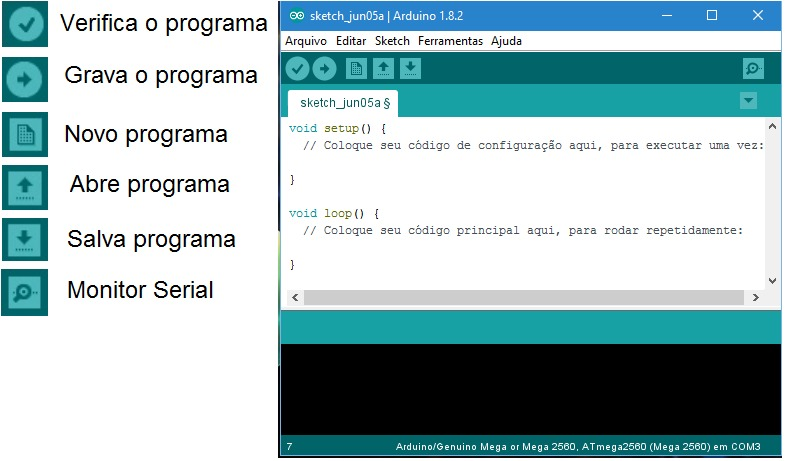
\includegraphics[width=.9\textwidth]{ide.jpg}
\caption{Interface da IDE do Arduino, Arduino IDE 1.8.2.}
\label{fig:exampleFig1}
\end{figure}
 Na (Figura 2) a placa ATmega 2560 utilizada no projeto e na (Figura 3) suas especificações técnicas.
\begin{figure}[ht]
\centering
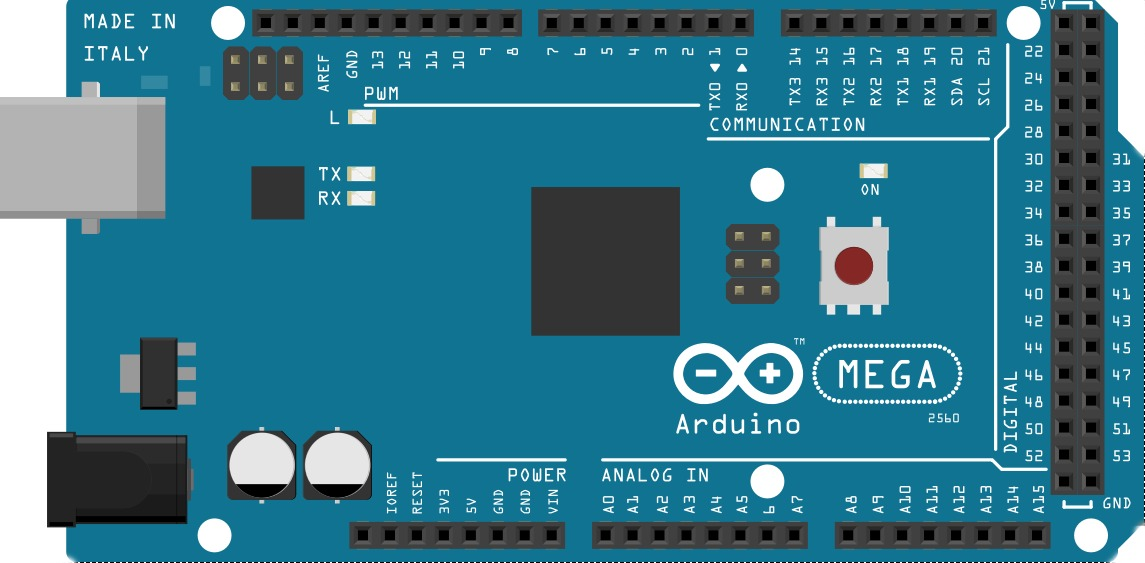
\includegraphics[width=.6\textwidth]{placa.jpg}
\caption{Placa Arduino ATmega 2560.}
\label{fig:exampleFig1}
\end{figure}

\begin{figure}[ht]
\centering
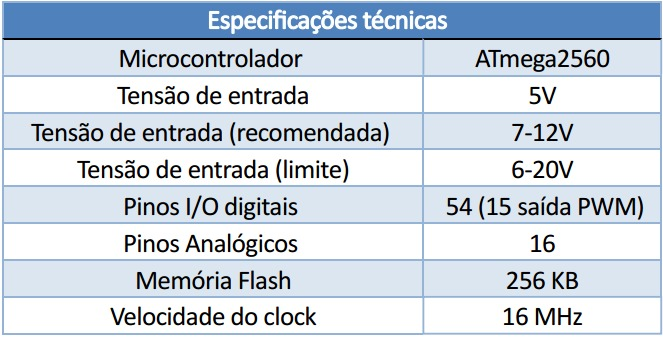
\includegraphics[width=.6\textwidth]{espplaca.jpg}
\caption{Especificações técnicas da placa.}
\label{fig:exampleFig1}
\end{figure}



\section{Metodologia}

\begin{itemize}
    \item Produção de um bafômetro controlado pela plataforma
Arduino.
    \item Realização de medições de concentrações de álcool no ar com
uma boa aproximação dos valores reais das concentrações.
    \item Exibir o valor adquirido em um Display de Cristal Líquido. o qual é a interface entre o motorista e o sistema.
\end{itemize}
\section{Drive Safe Detector}

O \emph{DSDetector}, um sistema embarcado projetado em \emph{C++},
utiliza o paradigma de programação orientado a objetos, feito
totalmente na plataforma \emph{Arduino}. Ele é composto por dois
periféricos de entrada, Sensor de gás \emph{MQ-3} e sensor de
Temperatura, três periféricos de saída, Display \emph{Lcd}, \emph{Buzzer
Beep} e Led Vermelho, e demais componentes.\\ \\ Ele é capaz de coletar a concentração de álcool no sangue do motorista através de sua respiração e do ar ambiente, realizando as compensações da temperatura ambiente, a qual necessita a utilização de um sensor de temperatura acoplado ao  sistema, e a partir do limite permitido pela Lei Seca que é de 0,3 mg/l de álcool no sangue, definir se o motorista esta ou não hapto a dirigir.
\subsection{Esquemático e Diagrama UML do Sistema}

Foi feito o esquema do Hardware do sistema assim como mostra a (Figura 4), onde mostra que o sistema estará acoplado à fonte de alimentação da ignição, ou seja, o sistema terá controle sobre a partida do veículo.

\begin{figure}[ht]
\centering
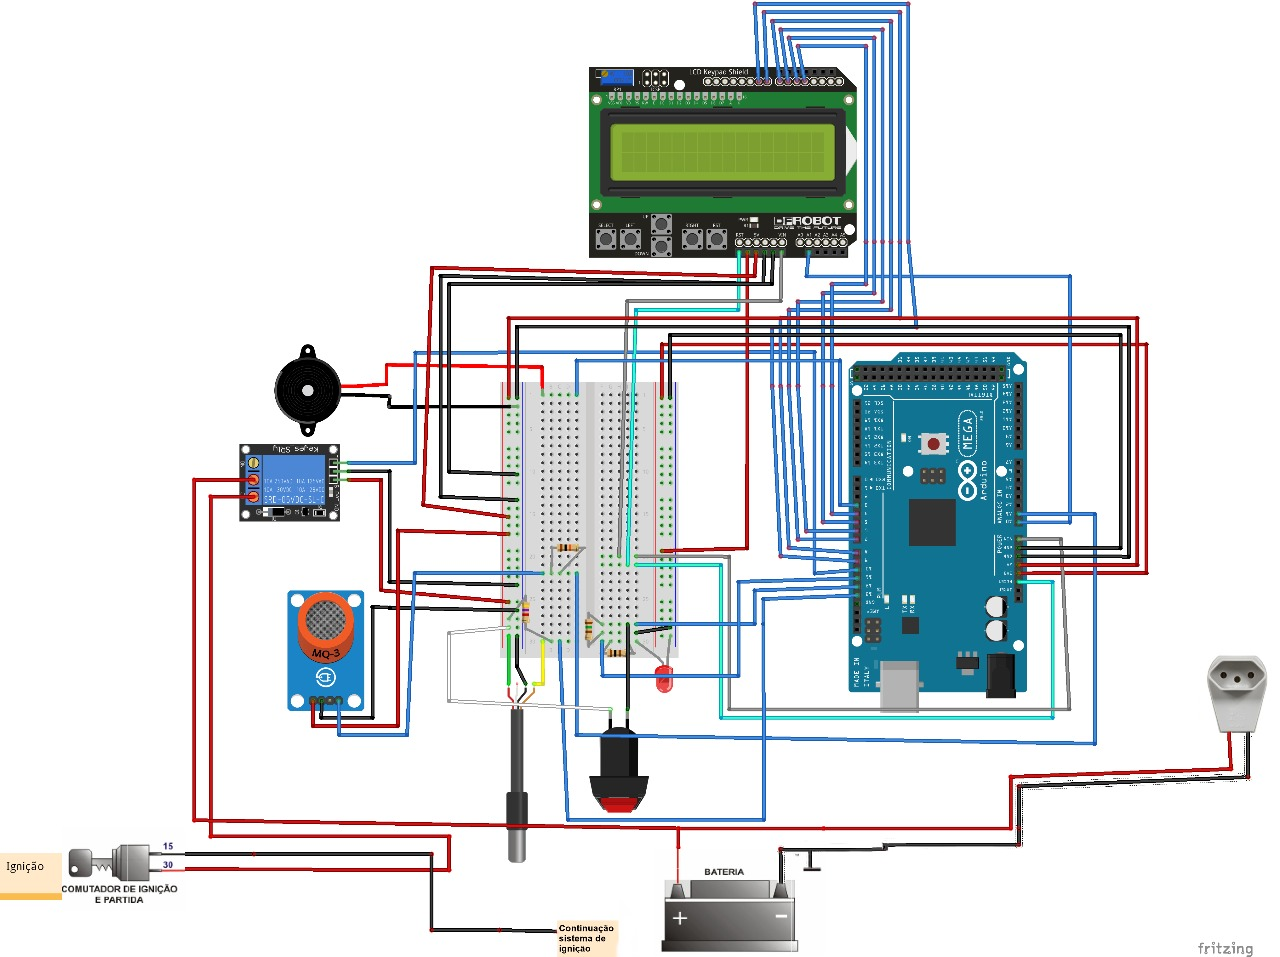
\includegraphics[width=.7\textwidth]{sistema.jpg}
\caption{Esquemático do sistema feito a partir da plataforma \emph{Fritzing}.}
\label{fig:exampleFig1}
\end{figure}

O diagrama UML do projeto dispõe as classes do projeto e suas relações, padrão tipicamente utilizado na programação orientada a objetos.
\begin{figure}[ht]
\centering
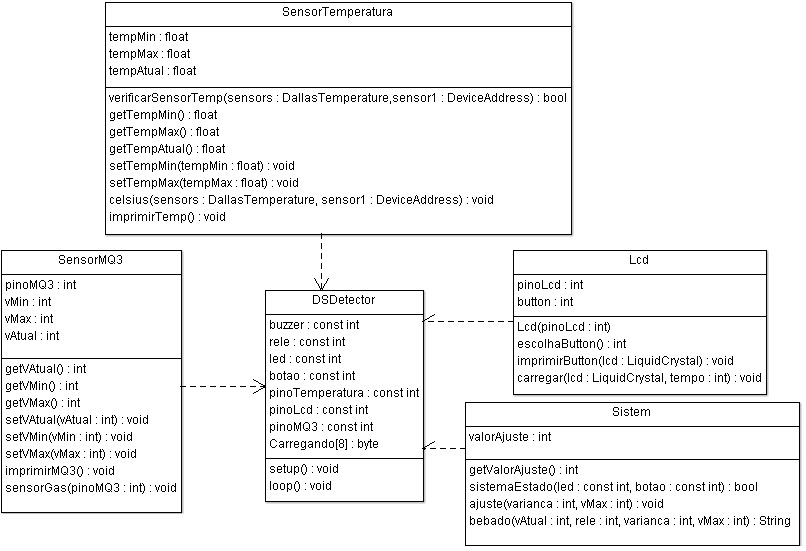
\includegraphics[width=.6\textwidth]{uml.jpg}
\caption{Diagrma UML do \emph{DSDetector}}
\label{fig:exampleFig1}
\end{figure}


\subsection{Como Funciona o Sistema}

\begin{itemize}
    \item O \emph{DSDetector}, será acoplado a um veículo tendo como fonte
de alimentação a bateria do veículo com tensão de 12v a qual
será regulada, a partir da montagen do sistema no veículo ele
será ligado, ficando em funcionamento por tempo
inderteminado, caso o motorista deslige o sistema ele não
poderá dar partida no veículo e o sistema acionara o \emph{Buzzer
Beep}.

\item Assim que ligado, o sistema terá um tempo para entrar em
operação, devido ao sensor \emph{MQ-3} que precisa ser aquecido,
tempo o qual irá variar de acordo com a temperatura
ambiente, após a inicialização o sistema estará em
funcionamento total.
\item Logo após a inicialização do sistema vai entrar em modo de
espera até que o motorista aperte o botão select, então o
sistema fará a primeira leitura de concentração de álcool na
respiração do motorista e a temperatura ambiente.

\item O sistema irá ficar verificando se o motorista ingeriu álcool ou
não, caso motorista tenha ingerido álcool o sistema não irá
permitir que o motorista ligue o veículo.

\item Logo após a primeira verificação o sistema irá rodar em
segundo plano, verificando se à álcool no ambiente e lendo a
temperatura para ajustar com a detecção de álcool no
ambiente.
\end{itemize}

\section{Testes e Resultados}

Foram feitas coletas de dados de acordo com os seguintes
intervalos de temperatura, temperatura menor ou igual a
19ºC, maior que 19ºC e menor que 27ºC e maior ou igual a
27ºC, intervalos os quais foram verificados mudanças na coleta
do sensor \emph{MQ-3}.


Podemos observar na (Figura 6) os valores do sensor \emph{MQ-3} de acordo com cada faixa de temperatura, logo após o aquecimento do sensor, o fator irá variar de acordo com os três intervalor de temperatura, a partir dele foi estabelecido um BrAc máximo, numa temperatura abaixo de 19ºC o \emph{DSDetector} irá alterar seu código estabelecendo o fator como sendo 0,004 mg/l, ou seja, caso o sensor tenha coletado um BrAc acima de 75ppm o BAC irá ultrapassar o limite permitido pela Lei Seca.
\begin{figure}[ht]
\centering
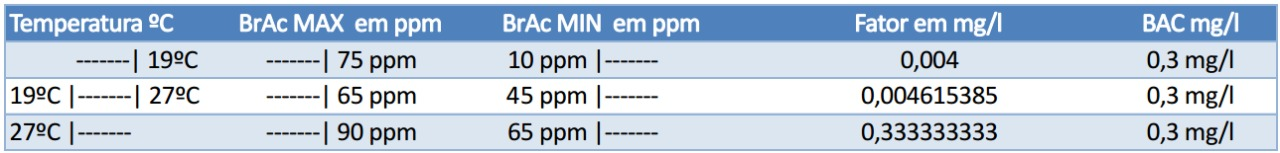
\includegraphics[width=.9\textwidth]{tabela1.jpg}
\caption{Tabela da primeira coleta de dados do sistema.}
\label{fig:exampleFig1}
\end{figure}

Depois da detecção de álcool o sensor \emph{MQ-3} leva um certo
tempo para restabelecer seus valores normais, então foi adotado um tempo padrão para restabelecimento do sensor de acordo com a temperatura, assim como mostra a (Figura 7).


\begin{figure}[ht]
\centering
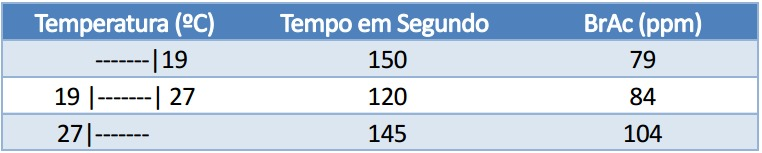
\includegraphics[width=.6\textwidth]{tabela2.jpg}
\caption{Tempo de restabelecimento do sensor.}
\label{fig:exampleFig1}
\end{figure}

Depois da detecção de álcool no sensor \emph{MQ-3} e a espera para
o mesmo se restabelecer o código sofre alteração devido a
forma despadronizada para a volta do valor inicial, sendo agora
os valores para detecção modificados.

\begin{figure}[ht]
\centering
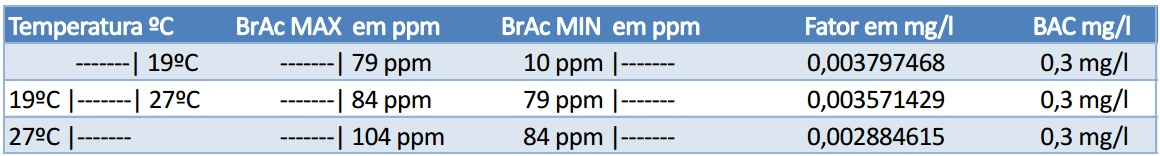
\includegraphics[width=.9\textwidth]{tabela3.jpg}
\caption{Tabela da segunda coleta de dados do sistema.}
\label{fig:exampleFig1}
\end{figure}

\section{Código Principal do Sistema}

\lstinputlisting{codigo.c}
\begin{thebibliography}{9}

\bibitem{datashettemp}
  Maxin Integrated, \emph{Programmable Resolution 1-Wire Digital Thermometer}. Disponível em:
  http://datasheets.maximintegrated.com/en/ds/DS18B20.pdf.
\bibitem{gitonewire}
  Paul Brook, \emph{Repositories GitHub, Arduino One-Wire library}. Disponível em:
  https://github.com/pbrook/arduino-onewire. 16 de outubro de 2012.
\bibitem{gitdallas}
 Miles Burton, \emph{Arduino Library for Maxim Temperature Integrated Circuits}. Disponível em:
  https://github.com/milesburton/Arduino-Temperature-Control-Library.\\ 11 de abril de 2017.
\bibitem{mq-3}
  Antony García González, \emph{Sensor MQ-3, un Detector de Alcohol}. Disponível em:
  http://panamahitek.com/sensor-mq-3/. 1 de fevereiro de 2014.
\bibitem{lcd}
  Arduino e Cia, \emph{Shield LCD 16x2 com Keypad}. Disponível em:
  http://www.arduinoecia.com.br/2013/08/arduino-shield-lcd-16x2-com-keypad.html. \\ 27 de agosto de 2013.
\bibitem{sistema}
  Guilherme Biff Zarelli, \emph{Arduino Sensor de Gás Detector de Gás (Arduino MQ Gas Sensor)}. Disponível em:
  http://helpdev.com.br/2013/07/07/arduino-sensor-de-gas-detector-de-gas-arduino-mq-gas-sensor/. 7 de julho de 2013.
\bibitem{placa}
  ARDUINO e GENUINO PRODUCTS, \emph{Arduino MEGA 2560 e Genuino MEGA 2560}. Disponível em:
  https://www.arduino.cc/en/main/arduinoBoardMega2560.
  \bibitem{iginicao}
  Saulo Anderson Bibiano Jardim, \emph{Como Funciona o Sistema de Ignição}. Disponível em:
  http://www.ebah.com.br/content/ABAAAA8pgAC/como-funciona-sistema-ignicao.
   \bibitem{git}
  Git, \emph{Git - Controle de Versões Rápidas}. Disponível em:
  https://git-scm.com/doc.
 \bibitem{argouml}
  Tigris.org Open Source Software Engineering Tools, \emph{ArgoUML Documentation}. Disponível em:
 http://argouml.tigris.org/documentation/. 29 de janeiro de 2011.
 \bibitem{github}
  GitHub Inc, \emph{The World's Leading Software Sevelopment Platform}. Disponível em:
 https://github.com/.
\bibitem{leiseca}
  Lei Seca, \emph{Lei Nº 11.705, de 19 de junho de 2008}. Disponível em:
 http://www.planalto.gov.br/ccivil03/ato2007-2010/2008/lei/l11705.htm.\\ 16  de junho de 2008.
\bibitem{leiseca}
 Inmetro, \emph{Etilômetro (Bafômetro) Controle pelo Inmetro}. Disponível em:
 http://www.inmetro.rs.gov.br/etilometro.html.
 \bibitem{conexaotemp}
  Blog FILIPEFLOP, \emph{Medindo temperatura debaixo d`água com DS18B20}. Disponível em:
  http://blog.filipeflop.com/sensores/sensor-de-temperatura-ds18b20-arduino.html.\\ 2 de junho de 2015.
\bibitem{arduinodocumentacao}
  Arduino IDE 1.8.2, \emph{Language Reference}. Disponível em:
  https://www.arduino.cc/en/Reference/HomePage. 
\bibitem{fritzaing}
  Fritzing Eletronics Made Easy, \emph{Fritzing References}. Disponível em:
  http://fritzing.org/learning/fullreference.
\end{thebibliography}
\bibliography{sbc-template}

\end{document}
